\documentclass[sigconf, review, anonymous]{acmart}

\usepackage{booktabs} % For formal tables
\usepackage{adjustbox}
\usepackage{color}
\usepackage{float}

\newcommand\Tstrut{\rule{0pt}{2.2ex}}         % = `top' strut
\newcommand\Bstrut{\rule[-0.7ex]{0pt}{0pt}}   % = `bottom' strut

% Copyright
\setcopyright{rightsretained}

%Conference
\acmConference[ESEC/FSE 2018]{The 26th ACM Joint European Software Engineering Conference and Symposium on the Foundations of Software Engineering}{4–9 November, 2018}{Lake Buena Vista, Florida, United States}

\begin{document}
\title{Bug Report Classification using LSTM architecture for \\More Accurate Software Defect Locating}

\author{Xin Ye}
\affiliation{%
  \institution{California State University San Marcos}
  \streetaddress{333 N Twin Oaks Valley Rd}
  \city{San Marcos}
  \state{California}
  \postcode{92069}
}
\email{xye@csusm.com}

\author{Fan Fang}
\affiliation{%
  \institution{California State University San Marcos}
  \streetaddress{333 N Twin Oaks Valley Rd}
  \city{San Marcos}
  \state{California}
  \postcode{92069}
}
\email{fang014@cougars.csusm.edu}

\author{Razvan Bunescu}
\affiliation{%
  \institution{Ohio University}
  \city{Athens}
  \state{Ohio}
  \postcode{45701}
}
\email{bunescu@ohio.edu}

\author{John Wu}
\affiliation{%
  \institution{California State University San Marcos}
  \streetaddress{333 N Twin Oaks Valley Rd}
  \city{San Marcos}
  \state{California}
  \postcode{92069}
}
\email{wu028@cougars.csusm.edu}

\author{Bartosh Sudak}
\affiliation{%
  \institution{California State University San Marcos}
  \streetaddress{333 N Twin Oaks Valley Rd}
  \city{San Marcos}
  \state{California}
  \postcode{92069}
}
\email{bartoshsudak@gmail.com}

\author{Hui Shen}
\affiliation{%
  \institution{Ohio University}
  \city{Athens}
  \state{Ohio}
  \postcode{45701}
}
\email{hs138609@ohio.edu}

\author{Chang Liu}
\affiliation{%
  \institution{Ohio University}
  \city{Athens}
  \state{Ohio}
  \postcode{45701}
}
\email{liuc@ohio.edu}

\begin{abstract}
Recently many information retrieval (IR)-based approaches have been proposed to help locate software defects automatically by using information from bug report contents. However, some bug reports that do not semantically related to the relevant code are not helpful to IR-based systems. Runing an IR-based system on these reports may produce false positives. In this paper, we propose a classification model for classifying a bug report as either helpful or unhelpful using a LSTM-network. By filtering our unhelpful reports before runing an IR-based bug locating system, our approach helps reduce false positives and improve the ranking performance. We test our model over 9,000 bug reports from three software projects. The evaluation result shows that our model helps improve a state-of-the-art IR-based system's ranking performance under a trade-off between the precision and the recall. Our comparison experiments show that the LSTM-network achieves the best trade-off between precision and recall than other classification models including CNN, multilayer perceptron, and a simple baseline approach that classifies a bug report based its length. In the situation that precision is more important than recall, our classification model helps for bug locating.
\end{abstract}

%
% The code below should be generated by the tool at
% http://dl.acm.org/ccs.cfm
% Please copy and paste the code instead of the example below.
%
\begin{CCSXML}
<ccs2012>
<concept>
<concept_id>10010147.10010257.10010258.10010259.10010263</concept_id>
<concept_desc>Computing methodologies~Supervised learning by classification</concept_desc>
<concept_significance>500</concept_significance>
</concept>
<concept>
<concept_id>10011007.10011074.10011099.10011102.10011103</concept_id>
<concept_desc>Software and its engineering~Software testing and debugging</concept_desc>
<concept_significance>500</concept_significance>
</concept>
<concept>
<concept_id>10002951.10003317.10003371.10003381.10003385</concept_id>
<concept_desc>Information systems~Multilingual and cross-lingual retrieval</concept_desc>
<concept_significance>300</concept_significance>
</concept>
</ccs2012>
\end{CCSXML}

\ccsdesc[500]{Computing methodologies~Supervised learning by classification}
\ccsdesc[500]{Software and its engineering~Software testing and debugging}
\ccsdesc[300]{Information systems~Multilingual and cross-lingual retrieval}


\keywords{Long short-term memory, convolutional neural network, bug locating, bug report}


\maketitle

\section{Introduction}
Software development is complex. During the software development and maintenance process, to ensure product quality, one of the most common tasks of a development team is bug fixing.

A software \textit{bug} or \textit{defect} is a coding mistake that may cause an unintended or unexpected behavior of the software component \cite{Bruegge:2009:OSE:1795808}. Upon discovering an abnormal behavior of the software project, a developer or a user will report it in a document, called a \textit{bug report} or \textit{issue report}. A bug report provides information that could help in fixing a bug, with the overall aim of improving the software quality. A large number of bug reports could be opened during the development life-cycle of a software product. For example, 3,352 bug reports of the Eclipse Platform product were submitted in 2016 alone\footnote{https://bugs.eclipse.org/bugs/}. In a software team, bug reports are extensively used by both managers and developers in decision making during their daily development activities \cite{Buse:2012:INS:2337223.2337343}. 

When a new bug report is received, before being solved, it will be screened and prioritized. This screening process is called bug report triage, which aims at ensuring the bug report quality. During the triage steps, the development team will check whether the bug report contains sufficient information for developers to fix, whether it is a duplicate report, what is its priority, and who should be the appropriate developer to solve it. After the triage, the report will be assigned to a developer to fix. Then the fix will be tested usually by another developer. If the fix is verified, the report will be closed. Otherwise, it will be assigned to someone again. This process represents a common defect cycle or bug-fixing cycle.

A developer who is assigned with a bug report usually needs to reproduce the abnormal behavior \cite{LaToza:2010:HQC:1937117.1937125} and perform code reviews \cite{Bacchelli:2013:EOC:2486788.2486882} in order to find the cause. However, the diversity and uneven quality of bug reports can make this process nontrivial. Essential information is often missing from a bug report \cite{Breu:2010:INB:1718918.1718973}. To locate the bug, developers not only need to analyze the bug report using their domain knowledge, but also collect information from peer developers and users to narrow their search. Employing such a manual process in order to find and understand the cause of a bug can be tedious and time-consuming \cite{Murphy-Hill:2013:DBF:2486788.2486833}. 

Bacchelli and Bird \cite{Bacchelli:2013:EOC:2486788.2486882} surveyed 165 managers and 873 programmers, and reported that finding defects require a high-level understanding of the code and familiarity with the relevant source code files. In the survey, 798 respondents answered that it takes time to review unfamiliar files. While the number of source files in a project is usually large, the number of files that contain the bug is usually very small. For example, the Eclipse JDT bug 424772 was fixed in a patch (commit) with four changed files, while the source code package checked out from this commit contains 10,544 Java files. Therefore, we believe that an automatic approach that ranked the source files with respect to their relevance for the bug report could speed up the bug finding process by narrowing the search to a smaller number of possibly unfamiliar files.

If the bug report is construed as a query and the source code files in the software repository are viewed as a collection of documents, then the problem of finding source files that are relevant to a given bug report can be modeled as a standard task in information retrieval (IR) \cite{Manning:2008:IIR:1394399}. In recent years, researchers \cite{Kim:2013:WFT:2554428.2554437, Lukins:2010:BLU:1824820.1824850, Nguyen:2011:TAN:2190078.2190181, Rao:2011:RSL:1985441.1985451, Saha:2013:ASE:6693093, Wong:2014:ICSME, Zhou:2012:BFM:2337223.2337226} have proposed various IR models to recommend source code files for bug reports automatically. These models use one or more \textit{features}. Each \textit{feature} is a type of information that measure the relationship between the bug report and the source code file. However, the weight parameters of these models are not learned automatically. Therefore, the feature combinations of these model are sub-optimal. The model scalability is also limited.

To address this issue, in preliminary work, the PI introduced a learning-to-rank model to combine different \textit{features} automatically \cite{Ye:FSE14, Ye:TSE15}. The problem of locating software defects is approached as a ranking problem, in which the source code files (documents) are ranked with respect to their {\it relevance} to a given bug report (query). In this context, {\it relevance} is equated with the likelihood that a particular source code file contains the cause of the defect described in the bug report. The ranking function is defined as a weighted combination of \textit{features}, where the \textit{features} are automatically trained on previously solved bug reports using a learning-to-rank technique. We performed extensive evaluations on six large open-source Java projects, from which the results showed that the learning-to-rank model outperformed other state-of-the-art approached \cite{Ye:TSE15, Ye:Dissertation}.

Matching bug reports with the relevant source code files is complicated by the lexical gap between natural languages used in the bug reports and the technical terms used in the source code files. To bridge this language mismatch, the PI employed word embeddings, which are vector representations of words, to measure the semantic similarity between bug reports and source code files \cite{Ye:ICSE16}. These semantic similarities are used as additional \textit{features} in the ranking function. Results of evaluations on four large open-source Java projects showed that adding these new word-embedding-based semantic features significantly improved the ranking performance \cite{Ye:ICSE16, Ye:Dissertation}.

\subsubsection{A.1 Objectives}
\label{sec:objectives}
The results of the PI's preliminary work are promising and motivate the PI to continue this work to address the following aspects.
\begin{enumerate}
  \item \textbf{Bug report quality classification:} Bug report quality varies. Some bug reports do not contain sufficient information for developers to locate the defect \cite{Breu:2010:INB:1718918.1718973}. Running a ranking system on low-quality reports may obtain misleading results. Therefore, the PI propose to include in the very beginning a pre-filtering step, in which a bug report is classified as either ``predictable'' or ``unpredictable''. After filtering out the ``unpredictable'' reports, the ranking system works only on the ``predictable'' reports and keeps silent otherwise. The purpose of doing so is to make the ranking results be more trustworthy. This project will use deep neural networks such as Convolutional Neural Network (CNN) \cite{LeCun:1989:BAH:1351079.1351090} and Recurrent Neural Network (RNN) \cite{Hochreiter:1997:LSM:1246443.1246450} for bug report classification.
  \item \textbf{Document-level similarity:} When calculating the word-embedding-based semantic features, our preliminary work used the Mihalcea's \cite{mihalcea:aaai06} similarity function, in which the similarity between a word $w$ in one document and a bag of words in another document $T$ is computed as the maximum similarity between $w$ and any word $w'$ in $T$: $sim(w, T) = \max_{w' \in T} sim(w, w')$. However, the similarities between $w$ and other words in $T$ are ignored, which cause information loss. As such, the PI propose to explore alternative methods for aggregating word-level similarities into a document-level similarity. More specifically, this project will use deep neural networks e.g. CNN and RNN to automatically learn feature vectors from bug reports and source code files respectively. Then a new semantic feature can be computed as the cosine similarity between the feature vectors of the bug report and a source file. This new feature can be used alone or as an complementary feature to improve the system performance.
  \item \textbf{User interface:} Despite many theories and algorithms were proposed recently to locate software defects automatically, practical systems with friendly user interfaces are rare, not to mention user studies that evaluate the effectiveness and usefulness of these approaches for developers in real work. Given the promising results of the preliminary work, which provides a self-learning ranking model on the back-end side, the PI propose to develop an interactive and user-friendly user interface on the front-end side. This project will develop a practical system that can be used in the software engineering course at California State University San Marcos (CSUSM) to help students better understand software engineering concepts.
\end{enumerate}

\subsection{B. Preliminary Work}
The preliminary work of this proposal produced the following results, which provide solid support for the proposed study.

\textbf{\underline{A learning-to-rank system}} \cite{Ye:FSE14,Ye:TSE15} was designed to rank all the source code files for a given bug report. Figure~\ref{fig:architecture} shows the high-level architecture of this system, in which the \textbf{ranking model} is trained to compute a matching score for any bug report $r$ and source code file $s$ combination. The scoring function $f(r, s)$, which is shown in Equation~\ref{eq:score}, is defined as a weighted sum of $k$ features, where each feature $\phi_i(r,s)$ refers to a measurement of the relation between the source file $s$ and the received bug report $r$:
\begin{figure}[t]
\centering
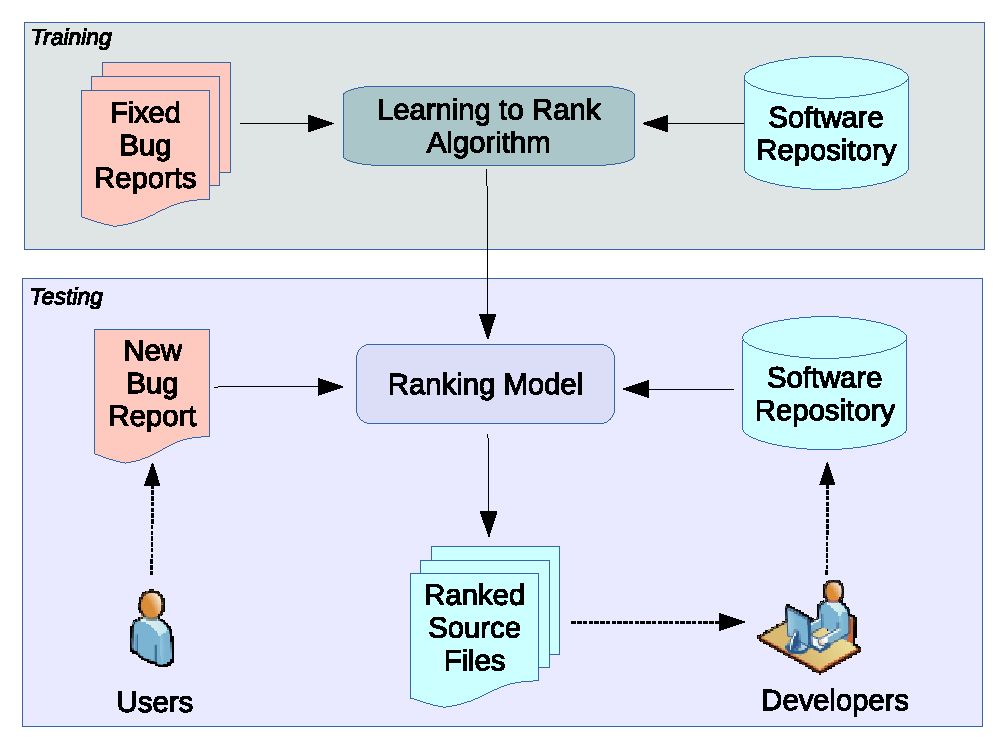
\includegraphics[width=\columnwidth]{figures/ye1.eps}
\caption{System architecture for {\it training} and {\it testing}.}
\label{fig:architecture}
\end{figure}
\vspace{-0.2em}
\begin{equation}
  f(r, s)= {\mathbf w}^T \Phi(r,s) = \sum_{i=1}^{k}w_i*\phi_i(r, s)
\label{eq:score}
\end{equation}
Given an arbitrary bug report $r$ as input at test time, the model computes the score $f(r, s)$ for each source file $s$ in the software project and uses this value to rank all the files in descending order. The user is then presented with a ranked list of files, with the expectation that files appearing higher in the list are more likely to be relevant for the bug report i.e., more likely to contain the cause of the bug.

The model parameters $w_i$ are trained on previously solved bug reports using a learning-to-rank algorithm \cite{Joachims:2006:TLS:1150402.1150429}. In this learning framework, the optimization procedure tries to find a set of parameters for which the scoring function ranks the files that are known to be relevant for a bug report at the top of the list for that bug report.

During feature engineering, we designed different types of features including features measuring the text similarity between bug reports and code in different granularity, features measuring the text similarity between bug reports and API references, features measuring the code change history, features about similar fix, and features measuring code complexity based on code-dependency graph \cite{Ye:TSE15}. The calculation of text similarity is based on the classic Vector Space Model (VSM) technique, which is widely use for measuring lexical similarity between documents. Later, to bridge the lexical gaps between bug reports and code, we used word embeddings, which are vector representations of words, to create two additional features for measuring their relations \cite{Ye:ICSE16}.

\textbf{\underline{A 3-D software visualization tool}} \cite{Ye:Access} was developed and was used for visualizing software project's \textit{Subversion} (SVN) repository. Figure~\ref{fig:teamwatch} shows a visualization view. Blue districts refer to folders. A stack of cylinders refers to a source code file. A single small cylinder refers to a revision of a source file. Different colors refer to different developers that contributed to the revisions.

\begin{figure}[t]
\centering
\includegraphics[width=\columnwidth]{figures/teamwatch.jpg}
\caption{Screenshot of a 3-D software visualization tool}%A 3-D Software Visualization (a) Revision statistics; (b) Developer statistics; (c) A single cylinder; (d) A stack of cylinders; (e) Filters; (f) Time Slider; (g) Blue district; (h) Transparent cylinders representing deleted files; (i) Return to the main menu.}
\label{fig:teamwatch}
\end{figure}

This visualization tool is too old to be used in the proposed study because 1) it works on a very old version control system SVN, which is seldom used now; 2) it visualized all the files of a project in one view, which causes poor poor scalability and can hardly work on large projects. However, its visualization scheme and the 3-D city metaphor will be used in the proposed study.

\subsection{C. Proposed Study}
The main goal of the proposed project is to develop an interactive and accurate software defect positioning system that can be used by developers to locate software defects efficiently. This practical system is a continuing work of the PI's preliminary work. To achieve the project goal, this project will pursue several objectives as discussed in Section A.1. More specifically, the PI propose to do the following work.

\subsubsection{C.1 Including a pre-filtering step to filter out ``unpredictable'' bug reports}
\begin{figure}[!h]
\centering
\includegraphics[width=\columnwidth]{figures/prefiltering.pdf}
\caption{Ranking after pre-filtering.}
\label{fig:prefiltering}
\end{figure}
Inspired by a similar work from Kim et al. \cite{Kim:2013:WFT:2554428.2554437}, the PI propose to include a pre-filtering step in the ranking system. The purpose is to further increase the ranking accuracy by filtering out ``unpredictable'' bug reports that do not contain sufficient information for locating the bug. As shown in Figure~\ref{fig:prefiltering}, a new received bug report will first be labeled by a classification model as either ``predictable'' or ``unpredictable''. Then the ranking system will rank all the source code files for a ``predictable'' report in order to locate the defect. But it will keep silent for ``unpredictable'' reports as it has no confidence in working correctly for this types of reports.

\begin{figure}[!h]
\centering
\includegraphics[width=\columnwidth]{figures/classification.pdf}
\caption{Bug report classification flowchart.}
\label{fig:classification}
\end{figure}
\begin{figure}[!h]
\centering
\includegraphics[width=\columnwidth]{figures/cnn.pdf}
\caption{An example of a CNN model.}
\label{fig:cnn}
\end{figure}

The flowchart of the classification model is shown in Figure~\ref{fig:classification}, where BR stands for bug report. The PI propose to use deep neural networks such as CNN and RNN. First, the content including summary and description of a bug report will be converted into a matrix of real numbers by using word embeddings. Next, CNN or RNN is applied on the BR matrix to learn a feature vector, which will serve as the input to a softmax regression model. The output is a label of either ``predictable'' or ``unpredictable''. The weight parameters of the softmax regression model is learned by using stochastic gradient descent on a dedicated training set with manually labeled bug reports. To create the training data, we will use the ranking results from the preliminary work \cite{Ye:ICSE16}. For a bug report in the training set, it will be label as ``predictable'' if the preliminary result \cite{Ye:ICSE16} successfully locate the bug within the top-10 ranked list, and it will be labeled as ``unpredictable'' otherwise.

Figure~\ref{fig:cnn} shows an example of a CNN model \cite{LeCun:1989:BAH:1351079.1351090} with two convolutional layers. The first convolutional layer uses a number of fix-size filters to perform convolution over the BR matrix and obtain the output of the same number of feature maps. Following is a max pooling layer that reduces the size of the feature maps. The output of the first layer serves as the input to the second convolutional layer. Finally, a fully connected layer produces a feature vector for the input BR matrix. It is noteworthy that when using CNN, all the training and testing BR matrices should have the same size. This can be done by extracting a fix size e.g. 100 words from all the bug reports. Reports with less words can be padded with 0. RNN works on input with variable length.

Recently, Mills et al. \cite{Mills:2017:PQQ:3092955.3078841} proposed an approach, which is based on the Lucene implementation of VSM~\footnote{https://lucene.apache.org/}, to predict query quality for assisting text retrieval tasks in software engineering. We will perform comparison with this related work and may use techniques from it to improve the proposed system.

\subsubsection{C.2 Introducing a new feature to measure the semantic similarity between bug reports and code}
In preliminary work, we use Mihalcea's function to aggregate word similarities into a document similarity. However, as discussed in Section A.1, it might cause information loss. Recently, Huo et al. \cite{Huo:2016:LUF:3060832.3060845} used CNN to to learn feature vectors from bug reports and code for measuring their similarity. But CNN requires fix-length input data and therefore may also cause information loss on code.

\begin{figure}[!h]
\centering
\includegraphics[width=\columnwidth]{figures/lstm.pdf}
\caption{Using LSTM to calculate similarity.}
\label{fig:lstm}
\end{figure}

The PI propose to use long short-term memory (LSTM) \cite{Hochreiter:1997:LSM:1246443.1246450}, a special type of RNN that can accommodate bug reports and source code files with variable length. Currently, LSTM networks are the most effective sequence learning models in many applications \cite{Goodfellow-et-al-2016}. We will use the standard LSTM unit defined in \cite{journals/corr/ZarembaSV14}. As shown in Figure~\ref{fig:lstm}, LSTM will be used to learn feature vectors from bug reports and source code files. The cosine similarity of their vector representations is considered as a measurement of their semantic similarity and will be used as a new feature in the ranking model.

\subsubsection{C.5 Evaluation}
We will evaluate the software defect positioning system on several large-scale open-source projects that contain a sufficient number (more than 2,000) of source code files and previously fixed bug reports. We will conduct experiments on software projects that are written in Java as well as projects written in C/C++ because these programming languages are widely used in both industry and academic. We will use projects from the Eclipse foundation~\footnote{https://eclipse.org/} and Apache foundation~\footnote{https://www.apache.org/} because 1) both have many large-scale open-source projects written in Java and C/C++; 2) the source code packages can be easily downloaded from their GIT repositories; 3) their bug reports or issue reports are public accessible. More specifically, the projects used in our preliminary work \cite{Ye:TSE15} will be used in this study. Additionally, we will run experiments on more projects such as Apache HTTP Server~\footnote{https://httpd.apache.org/} written in C, Lucene~\footnote{https://lucene.apache.org/} (an information retrieval software library) written in Java, and Hadoop~\footnote{http://hadoop.apache.org/} (a software framework for distributed storage and bigdata processing) written in Java. The selection of bug reports for evaluation is based on the same heuristics in \cite{Dallmeier:2007:EBL:1321631.1321702,Ye:FSE14}.

We will run the system to rank all the source code files for a given bug report and compare the result with the actual fix. The evaluation metrics such as \textit{Mean Average Precision} (MAP) \cite{Manning:2008:IIR:1394399} used in our preliminary work \cite{Ye:TSE15} will also be used in this study. Additionally, we will use Normalized Discounted Cumulative Gain (NDCG) \cite{Jarvelin:2002:CGE:582415.582418}, which is widely used in evaluating information retrieval models e.g. web search engines, to evaluate our system.

The PI is aware that user study is an effective way to evaluate the effectiveness of the proposed system in developers' real work. However, this is not the main goal of the proposed study. So the PI leave this to future work after the system is published. This study will also provide the basis for our future research on evaluating the effectiveness and usability of the proposed system in assisting teaching software engineering course at CSUSM.

\subsection{D. Work Plan}
The PI plan to hire one graduate student enrolled in the Master of Science Program in Computer Science (CS) and one undergraduate student enrolled in the Bachelor of Science in Computer Science program at CSUSM to help develop the system. The PI takes the overall responsibility of directing the project and keeps mentoring the students during the development.

\textbf{In the first year}, the graduate student will help implement the bug-report classification model, the LSTM-based semantic similarity feature, and the ranking model running on the server-side. The undergraduate student will implement the client-side programs and the web server that takes charge of the communication between the ranking model and the client-program. Since the ranking model, the database, and the web server work closely, the students will also work together closely during the development.

\textbf{In the second year}, two students will take charge of the maintenance and improvement of the system. Additionally, the graduate student will help run experiments to evaluate the ranking performance of the system on several open-source software projects, analyze the results, and improve the system accordingly. The undergraduate student will help develop a supplemental 3-D VR software visualization module. By the end of this year, the practical system will be published.

\textbf{Recruitment of students} will begin in spring, about three months before they start to work on the project. The PI will broadcast a hiring advertisement on CS-major electronic mailing lists, post a flier on class forums, and make a presentation of the project in the college-wide Frontiers in Science talk. In the coming 2017-2018 academic year, the CS department at CSUSM has a total of 866 undergraduate enrollments and a total of 39 graduate enrollments. Many students have desire to gain hands-on experience by working with faculty members on research projects. The PI will interview interested students. Preference will be given to economically-disadvantaged students, minority students, students making good progress toward their degree, and students who have demonstrated interest in this project.

\subsection{E. Broader Impacts}
The proposed study will result in a practical software system that alleviates develops' effort in bug finding and improves productivity. The system will be published. Any software developers can use and test it on their own projects. The system will be used in the software engineering courses at CSUSM to help students learn software engineering concepts in a lively manner. This project will expose students to an up-to-date software engineering research topic as well as some cutting-edge techniques including artificial neural networks and virtual reality.

The research outcome of this project will provide the basis for the PI's future research in performing user study and collecting user feedback to evaluate the effectiveness of the system in both academic and industry. The experience learned from this project will be very helpful for PI's research in code recommendation and automatic programming. The methodology and techniques used in this project will contribute to the software engineering research community.

The PI graduated with a Ph.D. degree from Ohio University at May 2016 and joined the CS department at CSUSM as an tenure-track faculty at August 2016. The funding to the proposed study will help the PI obtain important computing resources for building a software engineering (SE) research lab at CSUSM to continue his research. This fund, which supports two student assistants, will also help the PI found an SE research group at CSUSM. The research group will work on adapting new techniques to solve SE tasks, applying up-to-date SE research outcome to assist teaching SE courses, and engaging students in doing SE research projects.

The funding will have a significant impact on the quality of education for students here at CSUSM. The funds requested for student assistants will allow some of our economically-disadvantaged students, may of whom work in retail and on campus dining, to have paid positions during the academic year and summer.

Furthermore, funding of the proposed research program will create new opportunities for our students that have strong desire to participate in research projects. The research opportunities created from the funding of the proposed research will directly contribute to providing talented undergraduates at CSUSM with the research experience necessary to be competitive applicants for top-tier Ph.D. programs.

\begin{acks}
  The authors would like to thank Dr. Yuhua Li for providing the
  MATLAB code of the \textit{BEPS} method.

  The authors would also like to thank the anonymous referees for
  their valuable comments and helpful suggestions. The work is
  supported by the \grantsponsor{GS501100001809}{National Natural
    Science Foundation of
    China}{http://dx.doi.org/10.13039/501100001809} under Grant
  No.:~\grantnum{GS501100001809}{61273304}
  and~\grantnum[http://www.nnsf.cn/youngscientists]{GS501100001809}{Young
    Scientists' Support Program}.

\end{acks}

\section{Related Work}
\label{sec:related word}

Related work on word embedding in NLP was discussed in Section~\ref{sec:background}. In this section we discuss other methods for computing word similarities in software engineering and related approaches for bridging the lexical gap in software engineering tasks.

\subsection{Word Similarities in SE}

To the best of our knowledge, word embedding techniques have not been applied before to solve information retrieval tasks in SE. However, researchers \cite{Howard:2013:AMS:2487085.2487155, Wang:2012:ISR:2473496.2473617, 6224276} have proposed methods to infer semantically related software terms, and have built software-specific word similarity databases \cite{6747213, Tian:2014:SSW:2591062.2591071}.

Tian et al. \cite{6747213, Tian:2014:SSW:2591062.2591071} introduce a software-specific word similarity database called SEWordSim that was trained on StackOverflow questions and answers. They represent words in a high-dimensional space in which every element within the vector representation of word $w_i$ is the Positive Pointwise Mutual Information (PPMI) between $w_i$ and another word $w_j$ in the vocabulary. Because the vector space dimension equals the vocabulary size, the scalability of their vector representation is limited by the size of the vocabulary. When the size of the training corpus grows, the growing vector dimension will lead to both larger time and space complexities. Recent studies \cite{baroni-etal-2014b, Mikolov:ICLR} also showed that this kind of traditional count-based language models were outperformed by the neural-network-based low-dimensional word embedding models on a wide range of word similarity tasks.

Howard et al. \cite{Howard:2013:AMS:2487085.2487155} and Yang et al. \cite{6224276} infer semantically related words directly from comment-code, comment-comment, or code-code pairs without creating the distributional vector representations. They first need to map a line of comment (or code) to another line of comment (or code), and then infer word pairs from these line pairs. Similarly, Wang et al. \cite{Wang:2012:ISR:2473496.2473617} infer word similarities from tags in FreeCode. The main drawback of these approaches is that they rely solely on code, comments, and tags. More general free-text contents are ignored. Many semantically related words (e.g. ``placeholder'' and ``view'') are not in the source code but in the free-text contents of project documents (e.g. the Eclipse user guide, developer guide, and API document shown in Figure~\ref{fig:guide1} to Figure~\ref{fig:api}). However, these types of documents are not exploited in these approaches.

More importantly, all the above approaches did not explain how word similarities can be used to estimate document similarities. They reported user studies in which human subjects were recruited to evaluate whether the word similarities are accurate. However, these subjective evaluations do not tell whether and how word similarities can be used in solving IR tasks in SE.

\subsection{Bridging the Lexical Gap to Support \\Software Engineering Tasks}

Text retrieval techniques have been shown to help in various SE tasks \cite{Haiduc:2013:AQR:2486788.2486898, marcus2012use}. However, the system performance is usually suboptimal due to the lexical gap between user queries and code \cite{5989838}. To bridge the lexical gap, a number of approaches \cite{Bajracharya:2010:LUS:1882291.1882316, Chatterjee:2009:SSE:1533013.1533048, Dasgupta:2013:EST:2550526.2550586, 5989838, Stylos:2006:MWT:1174509.1174678, Ye:FSE14} have been recently proposed that exploit information from API documentations. These approaches extract API entities referenced in code, and use the corresponding documentations to enhance the ranking results.

Specifically, McMillan et al. \cite{5989838} measure the lexical similarity between the user query and API entities, then rank higher the code that uses the API entities with higher similarity scores. Bajracharya et al. \cite{Bajracharya:2010:LUS:1882291.1882316} augment the code with tokens from other code segments that use the same API entries. Ye et al. \cite{Ye:FSE14} concatenate the descriptions of all API entries used in the code, and directly measure the lexical similarity between the query and the concatenated document. The main drawback of these approaches is that they consider only the API entities used in the code. The documentations of other API entities are not used. Figure~\ref{fig:br1} shows the Eclipse bug 384108. Figure~\ref{fig:file} shows its relevant file {\it PartServiceImpl.java}. Figure~\ref{fig:api} shows the description of an API entry {\it IPageLayout}. Although {\it IPageLayout} is not used in {\it PartServiceImpl.java}, its API descriptions contains useful information that can help bridge the lexical gap by mapping the term ``view'' in bug 384108 with the term ``placeholder'' in {\it PartServiceImpl.java}. Therefore, to bridge the lexical gap, we should consider not only the descriptions of the API entities used in the code but also all API documents and project documents (e.g. the user guide shown in Figure~\ref{fig:guide1} and the developer guide in Figure~\ref{fig:guide2}) that are available.

Latent Semantic Indexing (LSI) and Latent Dirichlet Allocation (LDA) have been used in the area of feature location and bug localization. Poshyvanyk et al. \cite{Poshyvanyk:2007:FLU:1263152.1263534, Poshyvanyk:2006:CPR:1135772.1136177} use LSI to reduce the dimension of the term-document matrix, represent code and queries as vectors, and estimate the similarity between code and queries using the cosine similarity between their vector representations. Similarly, Nguyen et al. \cite{Nguyen:2011:TAN:2190078.2190181} and Lukins et al. \cite{Lukins:2010:BLU:1824820.1824850} use LDA to represent code and queries as topic distribution vectors. Rao et al. \cite{Rao:2011:RSL:1985441.1985451} compare various IR techniques on bug localization, and report that traditional IR techniques such as VSM and Unigram Model (UM) outperform the more sophisticated LSI and LDA techniques. These approaches create vector representations for documents instead of words and estimate query-code similarity based on the cosine similarity between their vectors. McMillan et al. \cite{Poshyvanyk:2013:CLU:2377656.2377660} introduced a LSI-based approach for measuring program similarity, and showed that their model achieve higher precision than a LSA-based approach in detecting similar applications. All these works neither measure word similarities nor try to bridge the lexical gap between code and queries.

\section{Conclusions and Future Work}
This paper introduces using a LSTM-network for classifying a bug report as either ``predictable'' or ``unpredictable''. While a ``pedictable'' report is considered helpful to an IR-based bug locating system to find the bug, an ``unpredictable'' report is deemed unhelpful to an IR system and is discarded. Evaluation results show that our classification model helps filter out ``unpredictable'' reports and improves the ranking performance of a state-of-the-art IR system on software bug locating. Among different classification models, the LSTM-network achieves the best trade-off between precision and recall. While our approach helps for IR-based bug locating, we observe the decrease of F1-Measure and the increase of F0.5-Measure. So we conclude that if precision and recall are given equal preference, our classification model is not helpful. But in the situation that precision is more important than recall, our classification model helps while keeping a certain trade-off between recall.

In future work, we will test the effectiveness of our approach using more IR-based bug locating systems on more software projects. In parallel, We plan to explore alternative methods like \textit{sent2vec} \cite{2017arXiv170302507P} for converting bug report into vector representations. Beside, we also plan to manualy review different bug reports to get insights of what type of quality make a report to be helpful to an IR system. We plan to create features that effectively represent the quality of bug reports and combine them with neural-network-based features for more precise classiication. 
\begin{acks}
  The authors would like to thank Dr. Yuhua Li for providing the
  MATLAB code of the \textit{BEPS} method.

  The authors would also like to thank the anonymous reviewers for
  their valuable comments and helpful suggestions.
\end{acks}


\bibliographystyle{ACM-Reference-Format}
\bibliography{bibliography}

\end{document}
